\documentclass[a4paper, 12pt]{report}
\usepackage{monapack}
\usepackage{hyperref}
\usepackage{amsmath}
\usepackage{numprint}
\npthousandsep{\,}
\usepackage[draft,nosingleletter]{impnattypo}


\newenvironment{absolutelynopagebreak}
{\par\nobreak\vfil\penalty0\vfilneg
\vtop\bgroup}
{\par\xdef\tpd{\the\prevdepth}\egroup
\prevdepth=\tpd}

\usepackage[outputdir=../]{minted}
\usepackage{xcolor}

\student{Ondřej Polanecký}
\trida{B4.I}
\obor{programator}
\bydliste{L. Janáčka 1266}
\datumNarozeni{3.1.2002}
\vedouci{Mgr. Milan Průdek}
\nazevPrace{Šachový bot}
\cisloPrace{23}
\skolniRok{2020/2021}
\reditel{Ing. Jiří Uhlík}

\zacatek

\titulniStrana


\anotace
Tato maturitní práce představuje můj šachový engine a vysvětluje některé techniky, které šachoví
boti využívají.
Také obsahuje GUI s~návodem na používání, aby si každý mohl snadno vyzkoušet zahrát si proti šachovému botu.
\newline\textbf{Klíčová slova:} Šachy, Šachový bot
\annotation
This graduation work presents my chess engine and explains some techniques used by chess engines.
It aslo contains GUI with guide how to use it, so everyone can easily play against my chess bot.
\newline\textbf{Keywords:} Chess, Chess bot, Chess engine
\podekovani
\obsah


\chapter{Úvod}
Tato maturitní práce představuje můj šachový engine a popisuje různé techniky a algoritmy používané v~šachových enginech.

V~této práci nebudu popisovat pravidla šachů, budu počítat s~vaší znalostí pravidel.


\chapter{Popis a struktura šachového enginu}


\section{Teorie her}


Šachy jsou stálé nevyřešená hra tzn. neví se jak vypadá bezchybná hra.
Jsou nevyřešené, protože počet možných pozic je enormní.
Už jenom po třech pohybech je \numprint{8902} možných variant hry.
Pro představu jsem vygeneroval graf pomocí programu Graphviz, který ukazuje jak se hra po třech tazích větví.
Viz obr.~\ref{fig:strom_tahu}
\begin{figure}
    \centering
    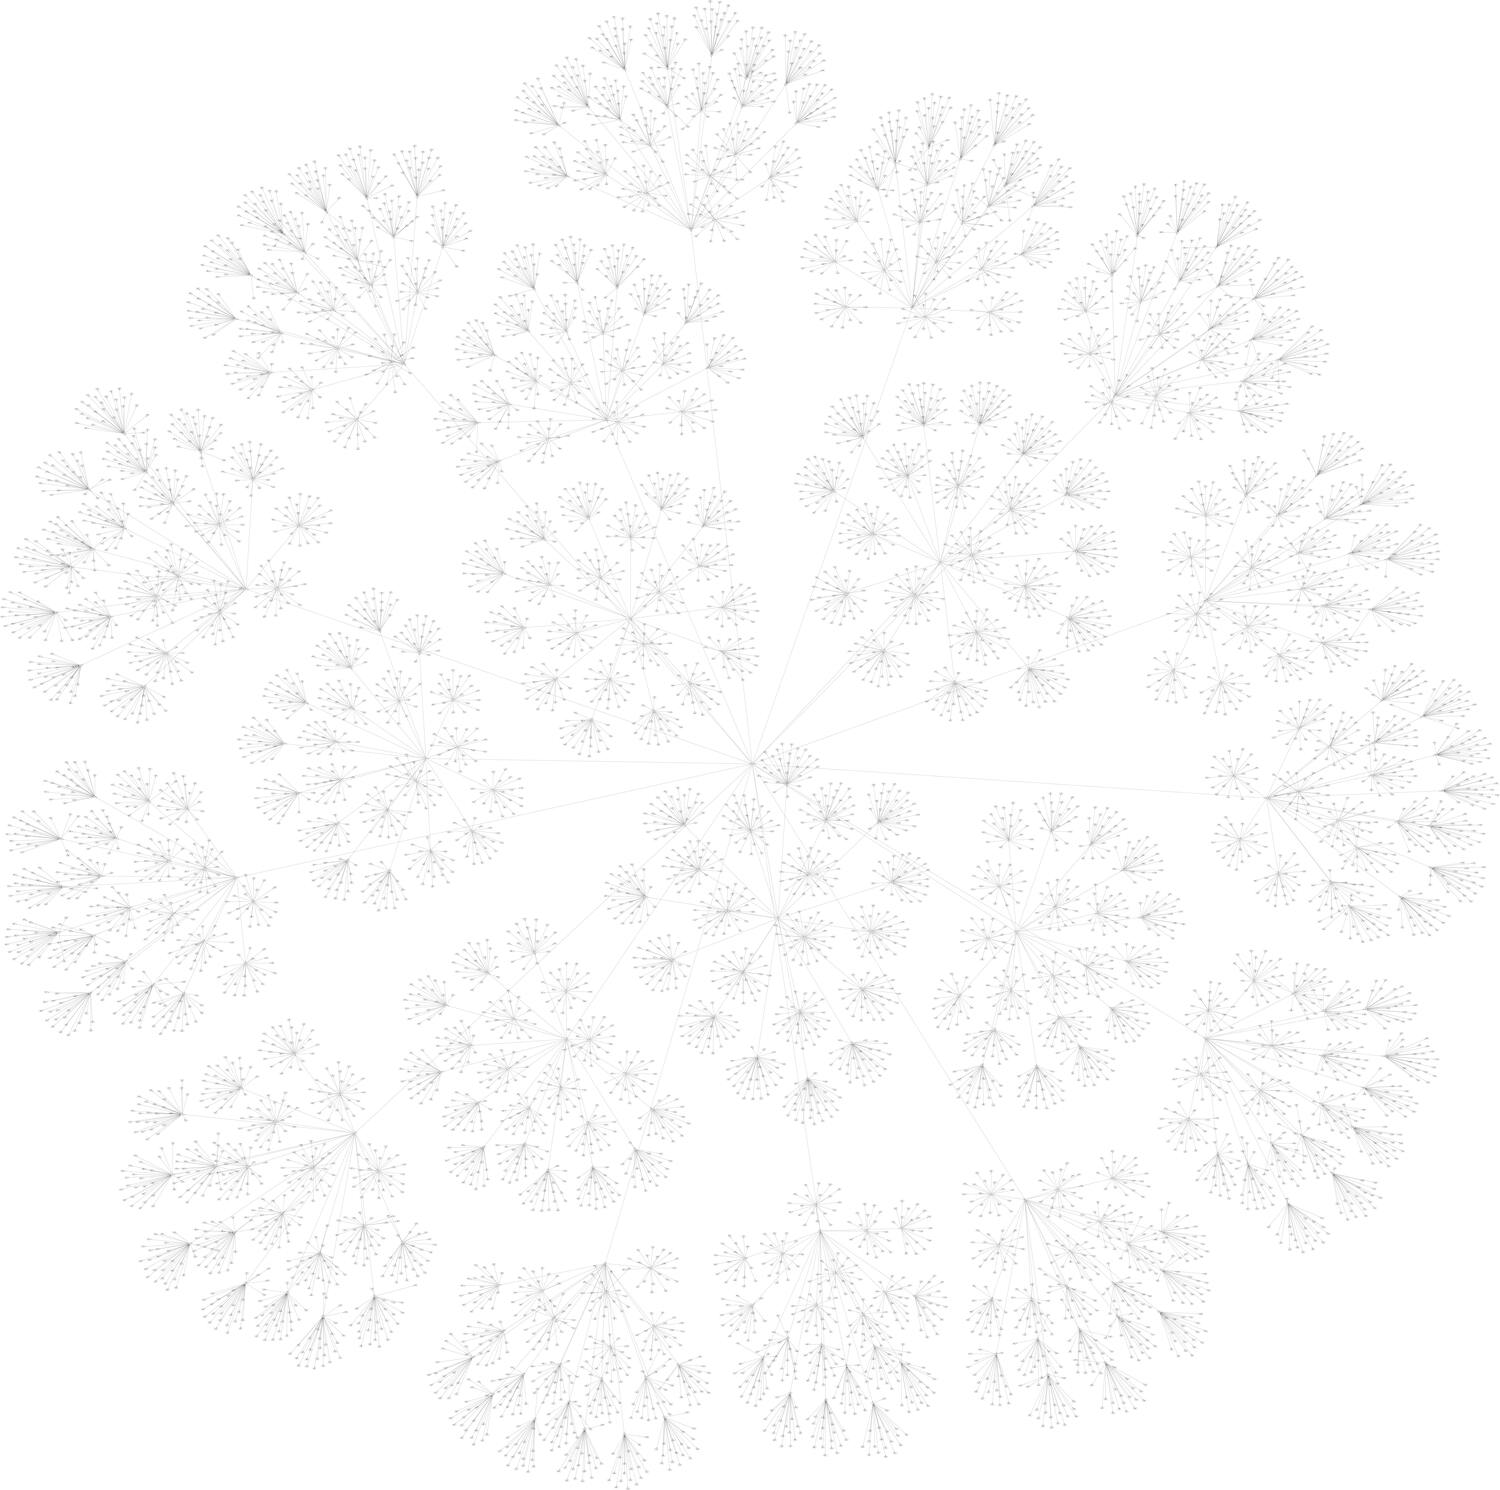
\includegraphics[scale=0.3]{images/graph.resized.jpg}
    \caption{větvění šachů po třech pohyběch}
    \label{fig:strom_tahu}
\end{figure}


Průměrný počet pohybů ve všech situací je přibližně 35,
průměrná hra má 80 pohybů, takže když chceme dostat hodně nepřesný odhad možných šachovým partií, tak nám stačí tyto dvě hodnoty umocnit
$35^{80} $\approx$ 10^{123} $\cite{shannon_number}.
Z~tohoto enormního čísla vyplývá, že šachy nelze vyřešit hrubou silou a pravděpodobně šachy v~nejbližší době, či dokonce nikdy nevyřešíme.
Pro zajímavost dáma má přibližně $5*10^{20}$ variací her a byla vyřešena v~roce 2007.\cite{dama} Při perfektním zahrání od obou hráčů skončí hra remízou.\newline
Šachy jsou:
\begin{itemize}
    \item  hra s~úplnými informacemi, tzn.
    oba hráči ví o~všech informacích ve hře (vidí všechny figurky).
    Na druhou stranu u~her s~neúplnými informacemi (např. poker),
    všechny informace neznáme a engine by musel počítat s~pravděpodobnostmi pro určité informace a na základě těchto pravděpodobností se rozhodovat.
    \item hra s~nulovým součtem, tzn. jakoukoliv výhodu hráč získá na úkor protihráče.
\end{itemize}
\begin{flushleft}
    Díky tomu můžeme tvořit herní strom všech možných tahů do určité hloubky a relativně dobře odhadovat hodnoty pohybů.
    Herní strom vypadá přibližně takto.
    Viz obr.~\ref{fig:game_tree}
    \begin{figure}
        \centering
        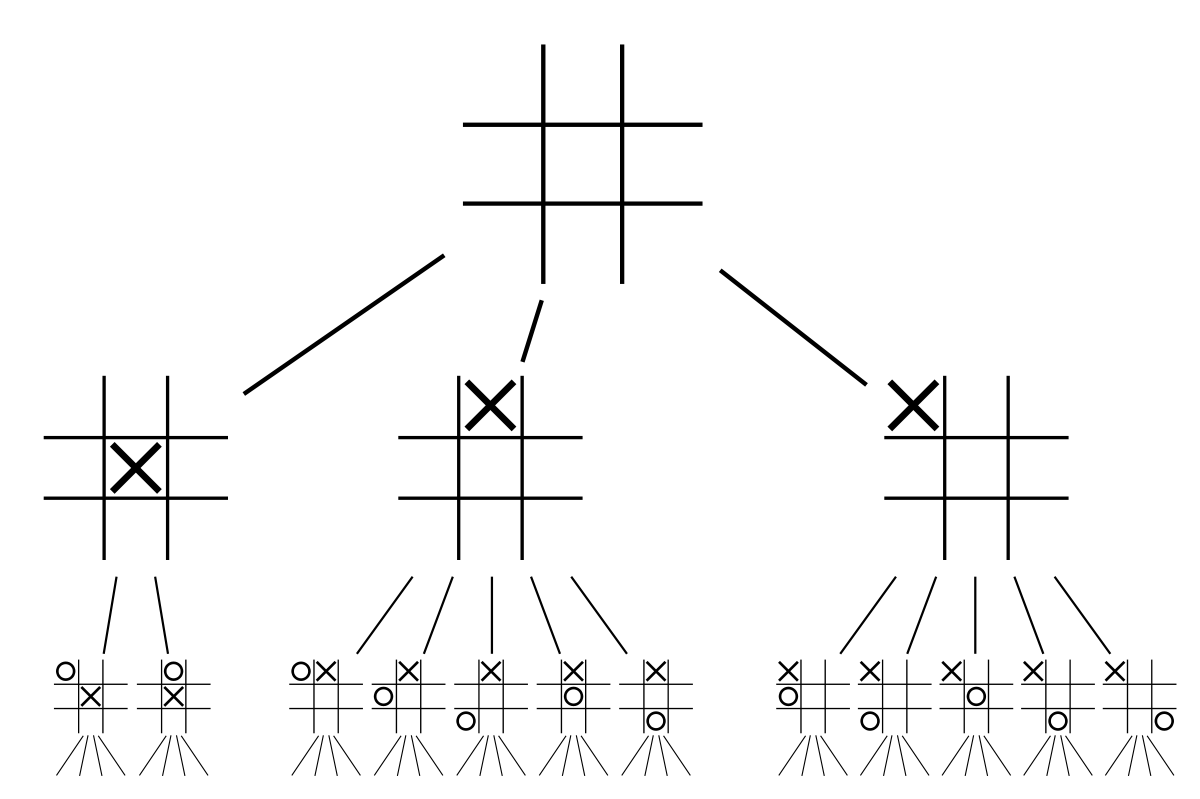
\includegraphics[scale=0.2]{images/game_tree}
        \caption{herní strom piškvorek~\cite{game_tree}}
        \label{fig:game_tree}
    \end{figure}

\end{flushleft}


\section{Dělení šachových enginů}
V~dnešní době existují v~podstatě dva druhy šachových botů.
\begin{itemize}
    \item Šachový bot založený na alfa-beta vyhledávání
    \begin{itemize}
        \item Šachový engine prochází rekurzivně herní strom do určité hloubky a na konečných uzlech stromu zhodnotí pozici.
        \item Hodnocení pozic je děláno funkcí vytvořenou programátorem a nedostatky evaluační funkce jsou dohnány prohledáváním spousty pozic do velké hloubky.
        \item Detaily budou v~kapitole~\ref{sec:alpha–beta-pruning}
    \end{itemize}
    \item Šachový bot založený na neuronových sítí a prohledávání stromu metodou Monte Carlo
    \begin{itemize}
        \item Šachový engine prochází rekurzivně herní strom do určité hloubky a na konečných uzlech stromu zhodnotí pozici.
        \item Hodnocení pozic je děláno neuronovou sítí, která byla natrénována na hraním proti sobě.
        \item Na vyhledávání se používá \href{https://en.wikipedia.org/wiki/Monte_Carlo_tree_search}{Monte-Carlo tree search}.
        Oproti Alfa-Beta vyhledávání prohledává podstatně méně pozic, ale prohledává pouze pozice s~velkou šancí na úspěšnost.
    \end{itemize}
\end{itemize}


\section{Struktura šachového enginu}\label{sec:struktura-šachového-enginu}
Můj šachový engine bude založen na alfa-beta vyhledávání, takže budu popisovat hlavně tento typ enginů.

Šachový engin by měl mít:
\begin{itemize}
    \item Generátor legálních pohybů
    \begin{itemize}
        \item Třída má na starosti generování legálních pohybů v~dané situaci
        \item Většina šachových enginů nejdřív vygeneruje všechny pseudo-legální pohyby\footnote{Pohyby, které odpovídají tomu, jak se mají figurky hýbat, ale je u~nich možnost, že by dostali svého krále do šachu.},
        otestuje pohyby a vyřadí u~kterých je vlastní král v~šachu.
    \end{itemize}
    \item Třída na reprezentaci stavu hry
    \begin{itemize}
        \item Udržuje informace o~pozicích, právech figurek a případně s~nimi hýbe
        \item na udržování pozic se většinou použivají bitboardy\footnote{Bitboard nebo bitmapa je 64 bitové číslo kde v~jeho binární podobně každá jednička znamená zabranou pozici na šachovém poli.}.
        Detaily o~bitboardech v~kapitole~\ref{sec:bitboard_kapitola}
    \end{itemize}
    \item Transpoziční tabulka
    \begin{itemize}
        \item Hašovací tabulka která obsahuje hashe pozic a nejlepší pohyb pro určitou pozici.
        \item Může obsahovat již prohledané pozice nebo pozice získané z~předem vytvořené databáze pohybů.
        \item Detaily v~kapitole~\ref{trans_tabulka}
    \end{itemize}
    \item Evaluace pozic
    \begin{itemize}
        \item Hodnotí pozici podle hodnoty, pozice a struktury figurek.
        \item Klíčová pro chování šachového enginu.
        \item Na základě ní se rozhoduje v~prohledávání pozic.
    \end{itemize}
    \item Prohledávací
\end{itemize}


\chapter{Implementace}\label{ch:implementace}


\section{Bitboardy}
\label{sec:bitboard_kapitola}

Bitboard je 64 bitové číslo.
Každá pozice bitu koresponduje s~pozicí na herní ploše.
Pokud je pozice na herní ploše zabrána, tak je korespondující bit v~bitboardu nastaven na 1.
Aby se dali rozlišit jednotlivé figurky, je třeba udržovat v~paměti bitboard pro každý druh a barvu figurek.
Viz. ilustrační obrázek \ref{fig:bitboard}
Důvod proč se využívají bitboardy je kvůli rychlosti generování pohybů.
Například u~generování pohybů pro koně jsme schopni si pro každou pozici předpočítat možné pohyby koně.
Také můžeme na bitboardy používat logické operace, takže můžeme například všechny pěšáky posunout o~8 bitů doprava (pohyb nahoru) v~jednom clock cyclu.
V~c++ jsem použil datovou strukturu unsigned long long.

\begin{figure}
    \centering
    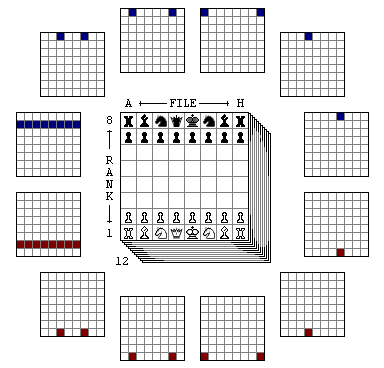
\includegraphics[scale=0.7]{images/bitboard}
    \caption{Reprezentace herní plochy pomocí bitboardů\cite{bitboards_wiki}}
    \label{fig:bitboard}
\end{figure}

\newpage

V~kódu udržuji bitboardy ve třídě Board.
Navíc k~tomu mám metody, které určité bitboardy spojí logickou operací OR.
Takhle vypadá definice třídy.

\begin{minted}[
    frame=lines,
    framesep=2mm,
    baselinestretch=1.2,
    fontsize=\footnotesize,
    linenos
]
{c++}
typedef unsigned long long bitboard;
class Board {
    public:
    bitboard all_bitboards[2][6]{};

    // spojene pozice

    // vraci bitboard figurek urcite barvy
    bitboard PiecesOfColor(bool color);

    // vraci bitboard vsech figurek
    bitboard AllPieces();
}
\end{minted}


\section{Generování pohybů}\label{sec:generování-pohybů}
Generování pohybů při používání bitboardů se dělá specifickým způsobem.
Pro figurky, které se hýbou nezávisle na tom kde jsou postaveny ostatní figurky, je to lehké.
Pouze pro všech 64 pozic kde se může figurka nacházet si předpočítáme možné pozice kam může jít.
Všechny tyto pozice uložíme do pole a jako index použijeme pozici bitu.
Když potom narazíme na figurku na určitém poli, stačí vzít předpočítaný bitboard.
Generování potom probíhá postupným procházení předpočítaného bitboardu.
Aby bylo procházení bitboardu co nejrychlejší používám funkci \_\_builtin\_ffsll().
Tato funkce je závislá na kompilátoru (GCC) a snaží se použít přímo assembly instrukci, pokud je dostupná.
Funkce vrátí velmi rychle index nejméně významného bitu, který je jedna.
Tím dostanu index pozice kam může figurka jít.
Prohledaný bit poté nastavím na nulu abych přístě dostal další jedničku.

Na ukázku přikládám úryvek kódu pro generování pohybů koňem.

\begin{minted}[
    frame=lines,
    framesep=2mm,
    baselinestretch=1.2,
    fontsize=\footnotesize,
    linenos
]
{c++}
    bitboard enemy_pieces = board.EnemyPieces();
    bitboard my_pieces = board.MyPieces();
    bitboard my_knights = board.all_bitboards[board.on_turn][KNIGHT];
    int from;
    int to;
    while (my_knights) {
        // nacteni pozice dalsiho kone
        from = __builtin_ffsll(my_knights);
        from--;
        // smazani nacteneho kone
        my_knights ^= 1ULL << (from);
        // utoky ze soucasneho kone
        bitboard attacks = precomp.precomputed_knights[from];
        // odstraneni pohybu, ktere by skoncili na nejake me figurce
        attacks &= ~my_pieces;
        while (attacks) {
            //nacteni pozice pro pohyb
            to = __builtin_ffsll(attacks);
            to--;

            // smazani nactene pozice
            attacks ^= 1ULL << (to);
            if (enemy_pieces >> to & 1ULL) {
                // pohyb sebere figurku
                moves.push_back(Move{from, to, KNIGHT, board.getPieceAt(to), true});
            }
            else {
                // pohyb nesebere figurku
                moves.push_back(Move{from, to, KNIGHT});
            }
        }
\end{minted}


Vetší problém je si předpočítat pohyby pro figurky u~kterých záleží na jakých pozicích jsou ostatní figurky (věž, střelec, dáma).
Je snadné
Když si vezmeme třeba tento příklad.\ref{fig:precomputed_rook1}
\begin{figure}
    \centering
    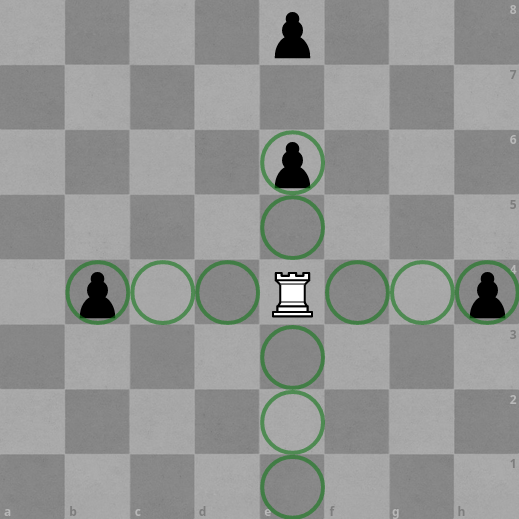
\includegraphics[scale=0.4]{images/precomputed_rook1}
    \caption{Možnosti pohybu věže}
    \label{fig:precomputed_rook1}
\end{figure}

Vidíme, že nás tedy zajímá jaké figurky blokují pohyb věže.
Můžeme si teda spočítat všechny možnosti kde můžou být.
Zajímají nás jenom figurky, které jsou na
V~tomto konkrétním případě je to 14 pozic kde můžou být figurky umístěny.
To je $2^{14}=16384$ pozic jak můžou být figurky uspořádány.
Dokonce to číslo můžeme ještě zmenšit, protože na úplně krajních pozicích nezáleží.
Krajní pozice totiž nic neblokují.
Takže v~tomto případě to je $2^{10} = \numprint{1024}$ pozic.
Což v~dnešní době není problém v~paměti udržet.
Teď ale musíme vyřešit jak budeme pozice v~poli indexovat.
Jedna možnost je použít hashmapu a jako index použít bitboard blokujících figurek.
Je tu ale rychlejší a paměťově méně náročnější možnost.
Jsou to tzv.
magické bitboardy.
Jde o~to, že v~celém bitboardu nás zajímají pouze určité bity.
A~my je můžeme rychlou metodou vyjmout z~bitboardu a indexovat pouze podle těchto určitých pozic.
Dělá se to tak, že se určitým číslem (magickým) vynásobí bitboard a to číslo je tak šikovné, že nám posune chtěné pozice na prvnich x bitů.
V~minulém případě by to posunulo těch 10 bitů na začátek čísla.
Pak jenom ořízneme zbytek bitboardu a indexujeme podle těchto 10 bitů.
Tyto čísla se získávají náhodným zkoušením a hledá se takové aby to namapovalo námi chtěné bity na co nejméně bitů.
V~ideálním případě na tolik bitů kolik bitů máme.
Já jsem si svoje čísla sám nepočítal.
Pouze jsem vzal čísla, které už někdo spočítal\cite{rustad-elliott}

Ukážu na příkladu jak by se vytvořil index pro tuto situaci.


\begin{minted}[
    frame=lines,
    framesep=2mm,
    baselinestretch=1.2,
    fontsize=\footnotesize,
]
{text}
bitboard bitů,                    bitboard obsazených                    bitboard
které nás zajímáají                      pozic                      blokujících figurek
. . . . . . . .                    1 1 . . . 1 . .                    . . . . . . . .
. . . 1 . . . .                    . 1 1 1 1 . . 1                    . . . 1 . . . .
. . . 1 . . . .                    . 1 . 1 . . . 1                    . . . 1 . . . .
. . . 1 . . . .                    . . . . . . . .                    . . . . . . . .
. 1 1 P 1 1 1 .         &          . 1 . . . . 1 .         =          . 1 . . . . 1 .
. . . 1 . . . .                    . . . 1 . . . .                    . . . 1 . . . .
. . . 1 . . . .                    . . . . . 1 . .                    . . . . . . . .
. . . . . . . .                    1 . . . . . . .                    . . . . . . . .

\end{minted}

Vezmeme bitboard bitů, které nás zajímají a provedeme bitový součin s~bitboardem obsazených pozic.
Tímto dostaneme bitboard blokujících figurek, který už máme vyřešený v~našem předpočítaném poli.
Jenom z~něho musíme dostat co je to za index.

\begin{minted}[
    frame=lines,
    framesep=2mm,
    baselinestretch=1.2,
    fontsize=\footnotesize,
    escapeinside=||,
]
{text}
 . . . . . . . .                                   |\colorbox{green}{1 1 . 1 . . 1 1}|
 . . . 1 . . . .                                   |\colorbox{green}{. .}| . 1 . . . .
 . . . 1 . . . .       pole magických čísel        . . . . . . . .
 . . . . . . . .                                   . 1 . . . . . .
 . 1 . P . . 1 .   *      rook_magic[P]       =    . . . . 1 . . .
 . . . 1 . . . .                                   . . . . . . . .
 . . . . . . . .                                   . . 1 . . . . .
 . . . . . . . .                                   . . . . . . 1 .
\end{minted}

Vynásobením magickým číslem dostaneme index.
Zeleně zabarvená část vypočítaného čísla je index.
Teď už jenom stačí bitovým posunem dostat jenom posledních 10 bitů čísla a máme index.

\subsection{Debugování}\label{subsec:debugování}
Problém s~debugováním generátoru pohybů je ohromné množství možných pozicí, takže je velmi obtížné hledat všechny chyby v~generátoru pouhým náhodným hraním.
Proto byl vymyšlen perft (PERFormance Test)\cite{perft}.
Perft projíždí všechny možné pozice do určité hloubky a konečné uzly stromu sečte.
Potom výsledek porovnám se známými správnými výsledky.
\newline
Výsledek spočítáme klasickým DFS (Depht First Search).
Budeme rekurzivně volat naší funkci na všechny pohyby a až dorazíme do hloubky jedna tak vrátímě počet všech pozic.
Ty se potom v~každé větvi sečtou.
Nakonec dostaneme všechny konečné pozice.
Tady je kód moji perft funkce.
\begin{minted}[
    frame=lines,
    framesep=2mm,
    baselinestretch=1.2,
    fontsize=\footnotesize,
    linenos
]
{c++}
unsigned long long perft(int depth, Board &board) {
    MoveGenerator gen = MoveGenerator();
    if (depth == 0) {
        return 1;
    }
    if (depth == 1) {
        return gen.getLegalMoves(board).size();
    }
    unsigned long long nodes = 0;
    for (auto move : gen.getLegalMoves(board)) {
        Board next_board = board;
        next_board.MakeMove(move);
        nodes += perft(depth - 1, next_board);
    }

    return nodes;
};
\end{minted}

Tuto funkci potom využiji na ověření správnosti generátoru takto.
Správné hodnoty konečných pozic jsem sebral z~internetu.\cite{perft_results}
Poté jsem jenom pomocí c++ knihovny Catch2 porovnal hodnoty.
\begin{minted}[
    frame=lines,
    framesep=2mm,
    baselinestretch=1.2,
    fontsize=\footnotesize,
    linenos
]
{c++}
    REQUIRE(perft(1, board) == 20);
    REQUIRE(perft(2, board) == 400);
    REQUIRE(perft(3, board) == 8902);
    REQUIRE(perft(4, board) == 197281);
    REQUIRE(perft(5, board) == 4865609);
    REQUIRE(perft(6, board) == 119060324);
\end{minted}


\section{Prohledávání pozic}\label{sec:alpha–beta-pruning}
Alfa beta prunning je metoda na zvolení nejlepšího pohybu ve stromu pohybů a odřezávání nepotřebných větví .
Je to vylepšení algoritmu minimax.

\subsection{Minimax}
Minimax algoritmus rekurzivně projde herní strom do nějaké hloubky a na posledním uzlu vrátí evaluaci pozice.
Při vracení rekurze vždycky porovnám všechny potomky pozice a vyberu tu nejvýhodnější pro hráče právě na tahu.

Takhle vypadá vygenerovaný minimax strom, který ještě nemá ohodnoceny poslední uzly.~\ref{fig:minimax_tree}

\begin{figure}
    \centering
    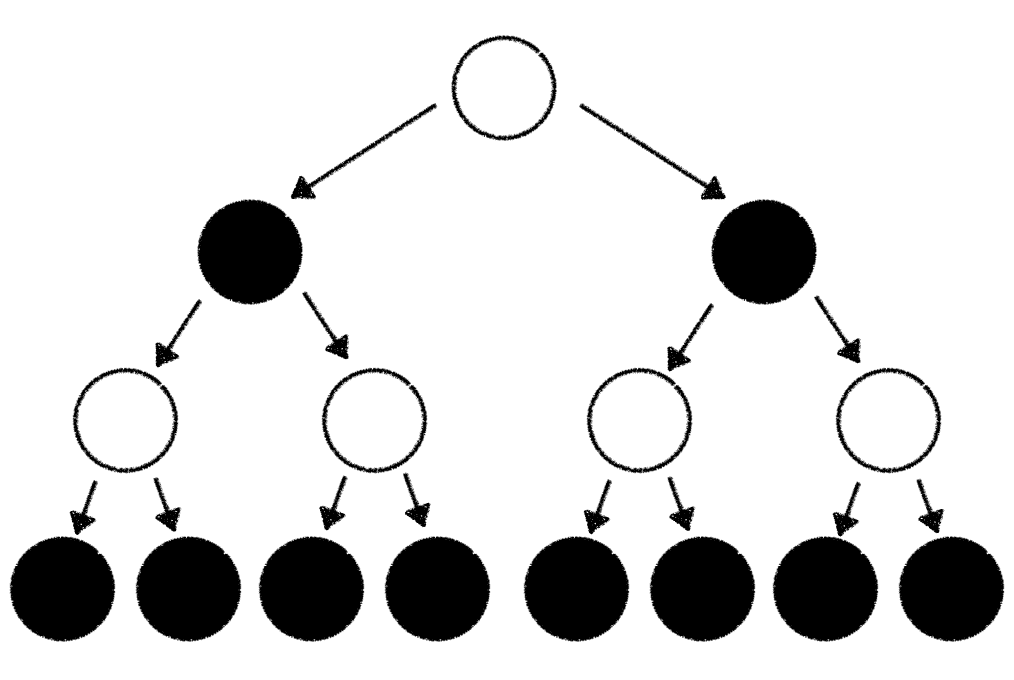
\includegraphics[scale=0.22]{images/minimax_tree}
    \caption{Minimax strom. Barva uzlu určuje hráče na tahu v~dané pozici}
    \label{fig:minimax_tree}
\end{figure}

Následně evaluační funkcí ohodnotím poslední uzly.\ref{fig:minimax_tree_last}
\begin{figure}
    \centering
    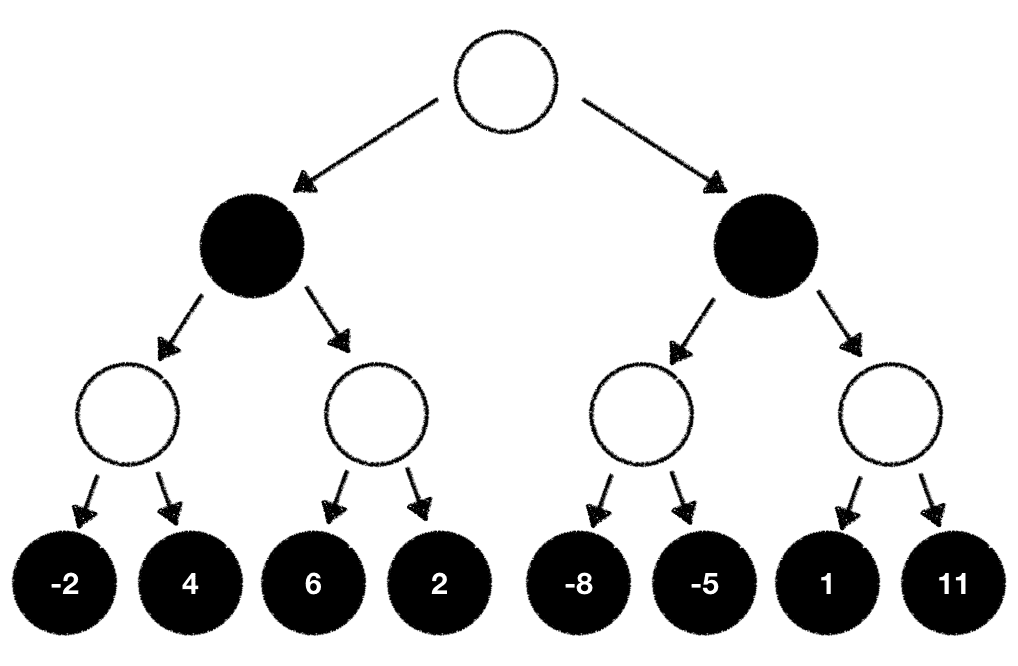
\includegraphics[scale=0.22]{images/minimax_tree_last}
    \caption{Minimax strom. Poslední pozice ohodnocené. }
    \label{fig:minimax_tree_last}
\end{figure}

Teď půjdeme zespodu nahoru.
Uzel porovná hodnoty všech potomků a nastaví svojí hodnotu na tu nejvýhodnější pro hráče na tahu.
Podle toho poté vybereme nejlepší pohyb.\ref{fig:minimax_tree_full}

\begin{figure}
    \centering
    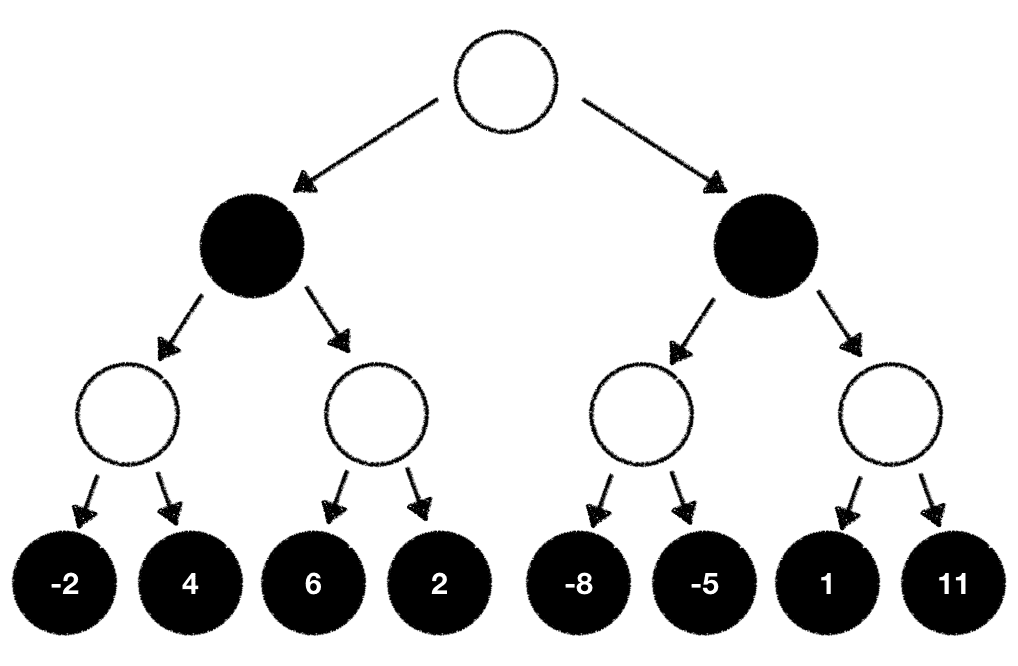
\includegraphics[scale=0.22]{images/minimax_tree_last}
    \caption{Minimax strom. Všechny pozice ohodnocené }
    \label{fig:minimax_tree_full}
\end{figure}

\subsection{Alpha-Beta pruning}\label{subsec:alha-beta-pruning}
Alpha-Beta pruning je vylepšení na algoritmu minimax.
Jde o~to, že není třeba vyhodnocovat všechny konečné uzly, protože při postupném vyhodnocování stromu zjistíme, že do některých větví se nikdy nemůžeme dostat za perfektního hraní nepřítele. Viz obr.\ref{fig:alpha_beta_full}
Abychom odřízli co nejvíce takovýchto větví, je klíčové pořadí pohybů.
Proto existují jsou různé techniky jak seřadit pohyby, aby nejvíce nadějné pohyby byli prozkoumány jako první.
Například pohyb z~transpoziční tabulky, sebrání nejcennější figurky nejméně cennou figurky a spoustu další heuristik pro dobré seřazení pohybů.\cite{move_ordering}



\begin{figure}
    \centering
    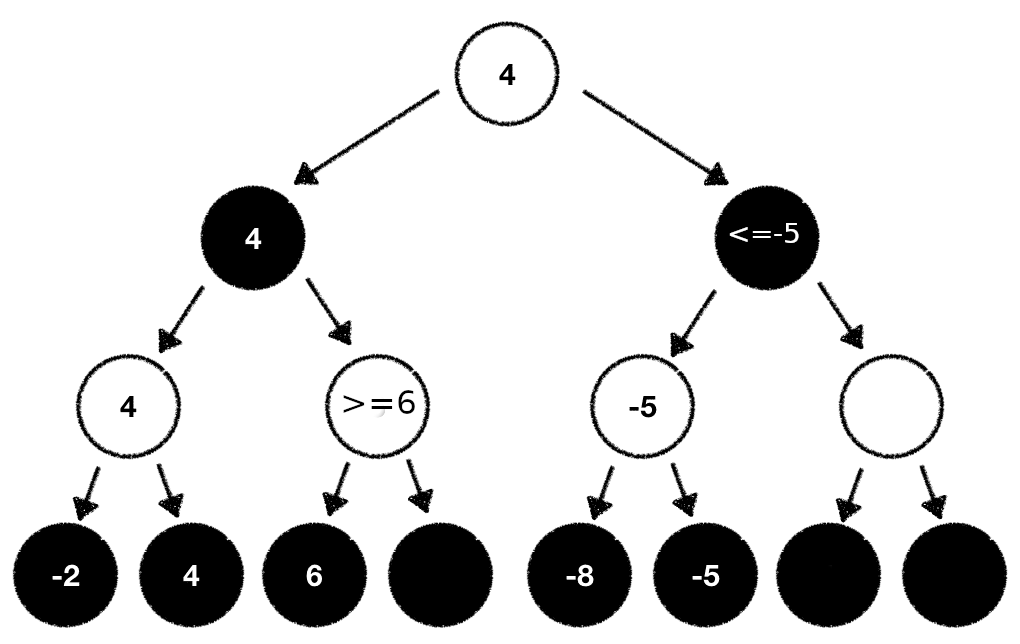
\includegraphics[scale=0.25]{images/alpha_beta_full.png}
    \caption{Ohodnocený strom pomocí alfa-beta pruningu. Prázdné uzly byli ořezány, jelikož je nebylo třeba prohledávat}
    \label{fig:alpha_beta_full}
\end{figure}


\section{Transpoziční tabulka}\label{sec:trans_tabulka}
Jelikož se často stává při prohledávání pozic, že narazíme na pozici, kterou už jsme někdy prohledávali, je výhodné si prohledané pozice ukládat.
V~c++ na to používám datovou strukturu unordered\_map, což je v~podstatě hashmapa, která má časovou složitost vkládání i čtení $O(1)$, díky čemuž je ideální na ukládání pozic.

\subsubsection{Zobrist hašování}
Jako klíč potřebuju vytvořit hash pozice, protože kdybychom použili všechny informace, museli bychom jako klíč použít 6 bitboardů plus informace o~en passantu, což je příliš.
Vzhledem k~tomu, že potřebujeme hash pozice vytvářet velmi často, je třeba aby hashovací funkce byla hodně rychlá.
Proto byla vytvořena metoda zobrist hashing\cite{zobrist1990new}.
Metoda se skládá ze dvou částí.

\begin{enumerate}
    \item Předpočítání náhodných čísel a zpočítání prvního hashe.

    Pro každý bit na každém bitboardu vytvořím náhodné 64-bitové číslo.
    Poté se vytvořím 64-bitové číslo kde budu udržovat hash pozice.
    Následně projdu všechny bitboardy a pro každý obsazený bit vyXORuju příslušné náhodné číslo na mojí hash pozici.
    Tím dostanu hash počáteční pozice.

    \item Aktualizování hash čísla podle zahraného pohybu.

    Krása zobrist hashování je, že když zpočítáme počáteční hash, můžeme poté hash pouze aktualizovat cca dvěma XOR operacemi.
    Když provedeme nějaký pohyb, potřebujeme z~hashe odstranit figurku která se pohla a přidat figurku tam kam se pohla.
    To uděláme tak, že použijeme náhodné hodnoty z~minulého kroku.
    Abychom figurku odstranili z~hashe, stačí nám na náš hash znovu vyXORovat náhodné číslo, které koresponduje s~touto figurkou na této pozici.
    Potom do hashe přidáme náhodné číslo, které koresponduje s~pozicí kam jsme figurku přesunuli.
\end{enumerate}

\subsubsection{Proč to funguje?}
Tato metoda funguje díky dvoum atributům XOR operace.
Zaprvé nám pomáhá asociativita XOR operace, tzn.\ že nezáleží na pořadí operací, což je přesně to co potřebujeme aby pozice měla stejný hash pokud se tam dostaneme různou variací pohybů.
Zadruhé nám pomáhá to, že XOR dvou stejným čísel je nula.
Takže když chceme z~hash čísla odstranit nějakou figurku, tak pouze na náš hash vyXORujeme náhodné číslo korespondující s~pozicí figurky.


\section{Databáze otevíracích pohybů}\label{sec:databáze-pohybů}
Počáteční fáze šachů je v~dnešní době prozkoumána do velké hloubky, takže naše znalosti mnohem převyšují schopnosti šachového najít nejlepší pohyby.
Proto je vhodné mít nějakou databázi pohybů, kterou použijeme na začátku hry.
Abych si vytvořil svojí databázi musím stáhnout nějakou sadu her.
Vybral jsem si sadu her MillionBase 2.5\cite{chess_database}, což je databáze 2.5 milionu kvalitních šachových partií ve formátu PGN\cite{pgn_format}.

\subsection{PGN formát}
PGN je standardní formát na zaznamenání her v~šachách.
Je relativně snadno čitelný pro lidi, ale není tak snadné ho počítačově zparsovat, protože není možné vytvořit pohyb bez znalosti stavu hry.
Jde o~to, že v~pgn formátu se používá co nejméně informací na identifikaci figurky kterou chceme hýbat.
Takže například pokud chceme v~PGN formátu zapsat, že chceme pohnout koněm na určité místo, a máme koně pouze jednoto, tak zapíšeme jenom že hýbáme koněm a kam s~ním hýbáme.
To, kterým koňem a odkud hýbáme vyplívá z~toho, že máme koňe pouze jednoho.
Pokud máme dva koňě, tak bychom k~tomu museli ještě připsat v~jakém sloupci, či řádku se nachází.
Takhle vypadá ukázková hra v~PGN formátu.


\begin{minted}[
    frame=lines,
    framesep=2mm,
    baselinestretch=1.2,
    fontsize=\footnotesize,
]
{text}
[Event "Spring "]
[Site "Budapest open"]
[Date "1996.??.??"]
[Round "1"]
[White "Aadrians, M. (wh)"]
[Black "Dekic, J. (bl)"]
[Result "0-1"]
[BlackElo "2320"]
[ECO "D82"]

1. d4 Nf6 2. c4 g6 3. Nc3 d5 4. Bf4 Bg7 5. Be5 dxc4 6. e3 Nc6 7. Qa4 O-O
8. Bxf6 Bxf6 9. Bxc4 a6 10. Bd5 b5 11. Qd1 Bb7 12. a3 e6 13. Bf3 Na5
14. Bxb7 Nxb7 15. b4 c5 16. bxc5 Nxc5 17. Nf3 Qa5 18. Qc2 Na4 19. Rc1 Rac8
20. O-O Qxc3 21. Qe2 Qxa3 22. Rc2 Rxc2 23. Qxc2 Qc3 24. Qe4 Rc8 25. g3 Qc2
26. Qb7 Qc6 0-1
\end{minted}
Svůj PGN parser\footnote{Parser je program na překlad určitého vstupu do žádaného výstupu. V~mém případě chci přetvořit PGN formát do struktury kterou používám na ukládání pohybů} chci mít co nejjednodušší, takže budu ignorovat informační tagy\footnote{Nad každou hrou. Obsahují metadata o~hře. Například ELO hráčů, či místo konáni hry.} a budu prohledávat maximálně do hloubky 14 pohybů.
Abych nemusel pokaždé před začátkem programu parsovat 2.5 miliónu her, napsal jsem si svojí takovou databázi a budu tedy vysledky ukladat do souborů.
Nejdříve si načtu všechny pohybu do datové struktury map<bitboard, unordered\_map<string, int>{}> , což je seřazená hash mapa podle klíče, která obsahuje neseřazenou hashmapu pohybů s~jejich četnostmi.
Abych efektivně tuto datovou strukturu využil i ze souboru, vytvořil jsem si datový a indexový soubor.
Indexový soubor obsahuje seřazené hash pozice a index pohybů pro určitý hash v~datovém souboru.
Datový soubor obsahuje na každém řadku všechny pohybý které byli v~dané pozic zahrány a jejich četnost.

Když budu chtít vyhledat zahrané tahy pro určitou pozici.
Vyhledám pomocí binárního vyhledávání hash v~indexovém souboru.
Tím dostanu pozici pohybů v~datovém souboru a podle této pozice tyto pohyby načtu.
Časová složitost vyhledávání bude

\[
    O(\log n + m)
\]
kde $n$ je počet hash pozic uložených v~indexovém souboru a $m$ je počet různých zahraných tahů v~určité pozici.


Tady je útržek kódu z~mého parseru.
\begin{minted}[
    frame=lines,
    framesep=2mm,
    baselinestretch=1.2,
    fontsize=\footnotesize,
    linenos
]
{c++}
depth++
database[board.zobrist_hash][token]++;
board.MakeMoveFromPGN(token);
\end{minted}
Je to kód ze smyčky která prochází už pohyby pgn formátu, které jsou uložené jako string ve proměnné tok.
Nejdřív zvětším hloubku prohledávání o~jednu.
Potom přidám jedničku ke četnosti pohybu, který se chystám zahrát v~dalším příkazu.


\chapter{GUI}\label{sec:gui}
Pro vytvoření GUI\footnote{Graphical User Interface} mého programu jsem zvolil OLC::PixelGameEngine\cite{olc_engine}, protože už jsem v~něm pracoval, je minimalistický a rychlý.
Vzhledem k tomu, že můj hlavní cíl mojí práce není GUI a bylo by časově náročné dělat nějaké propracované GUI, tak jsem ho vytvořil pouze na hraní za bílého a bez jakéhokoliv menu.
V PixelGameEnginu neexistují žádné běžné GUI prvky, pouze můžu kreslit tvary, obrázky a samotné pixely.
Vždycky, když se něco změní na hrací ploše, tak ji vykreslím celou znova.
Jediné co dělám je, že při kliku na figurku zvýrazním všechny možné tahy s touto figurkou a při kliku na nějaké místo tou figurkou táhnu.
Když zahraje tah člověk, začne s počítáním tahu počítač.
Přibližné prvních 5 bude velmi rychlých, protože jsou zahrány z databáze tahů.
Poté je na to engine sám a musí používat vyhledávací funkci.
Je důležité aby GUI beželo v jiném vlákně než vyhledávací funkce, protože jinak by GUI přestalo reagovat.
Mám jednu atomic\footnote{atomic proměnná v c++ znamená, že k ní nemůžou dvě vlákna přistoupit zároveň} proměnnou, která rozhoduje v jaké fázi je program, tedy jestli je na řadě bot, či hráč.


\section{Závěr}\label{sec:závěr}
Cílem mojí maturitní práce bylo vysvětlitp


\seznamTabulek

\seznamObrazku

\prilohy{
    \kapitola{Příloha}
}


\bibliographystyle{czechiso}
\bibliography{zdroje}

\konec

